%!TEX root = ../main.tex
\section{Appearance-based loop detection (Sonar Context)}
\label{sec:chap2}

The remaining weak point of chapter~1 is the \textbf{detection} of revisits: the
covariance-based preselection goes blind as soon as the accumulated uncertainty
grows. We replace this detection with \textbf{appearance-based} place recognition
derived from Sonar Context~[2], keeping the whole downstream geometric verification
(shgo + ICP + PCM) and the USBL anchoring of chapter~1 — a single stage changes in
figure~\ref{fig:pipeline}.

\subsection{Descriptor: Sonar Context re-derived for the P900}
\label{sec:sc-desc}

Sonar Context~[2] encodes the polar sonar image into an azimuth $\times$ range matrix
by intensity \emph{max-pooling}. On the Aracati P900 (low resolution, bright seabed,
saturations), max-pooling saturates everywhere: the descriptor does not discriminate
(\textbf{AUC 0.55}, measured on a bench of true/false revisit pairs). The retained
variant encodes the \textbf{density of structural returns}: the re-polarised image
$I$ is thresholded then block-averaged into $A \times R$ cells ($A = R = 40$):
\begin{equation}
C(a, r) = \frac{1}{|B_{a,r}|} \sum_{(u,v) \in B_{a,r}} \max\big(I(u,v) - \tau_I,\ 0\big),
\qquad \tau_I = 95
\end{equation}
normalised by its maximum. This variant separates true and false revisits well
(\textbf{AUC 0.86}). The \textbf{Polar Key} $P_r = \frac{1}{A}\sum_a C(a,r)$
(azimuth-invariant, hence heading-invariant) serves as a fast search index
(Euclidean kNN, $k = 5$).

\subsection{Distance and decision}
\label{sec:sc-dist}

Two contexts are compared with a column-wise cosine distance, minimised over bounded
shifts (rotation $\leftrightarrow$ azimuth shift, radial translation
$\leftrightarrow$ range shift), with \emph{zero-padding} (the 130° field of view is
not circular, unlike the Scan Context LiDAR):
\begin{equation}
d(C^q, C^c) = \min_{|s_a| \le 10,\ |s_r| \le 5}\ \frac{1}{R} \sum_{r}
\left(1 - \frac{\langle C^q_{\cdot r},\ \tilde{C}^c_{\cdot r}(s_a, s_r)\rangle}
{\lVert C^q_{\cdot r}\rVert\,\lVert \tilde{C}^c_{\cdot r}\rVert}\right)
\end{equation}
A candidate is retained if $d < \tau$ \textbf{and} if it passes a 10 m
\textbf{geometric gate} on the estimated pose distance (it removes the distant false
positives that appearance alone cannot rule out in a repetitive marina). The optimal
shift $(s_a, s_r)$ additionally provides a coarse initialisation of the
transformation.

\textbf{Threshold calibration.} The descriptor bench gives a Youden threshold at
0.695 (TPR 84~\%, FPR 24~\%). The decision log of a run
(\texttt{loops\_detected.csv}) then showed that between $\tau = 0.60$ and $0.70$
there were \textbf{+108 candidates, all true (0 false)} — with the geometric gate and
the PCM filtering downstream, we set $\tau = 0.70$ (116 loop constraints in the
graph, against 82 at 0.60).

\subsection{Geometric verification and anchoring unchanged}

Each retained candidate follows exactly the Bruce-SLAM pipeline~[1]: global shgo
initialisation (bounds capped at $\pm$20 m — without this cap, the accumulated
covariance inflates the bounds to $\pm$130 m and the optimiser no longer converges),
ICP with covariance, then pairwise consistency PCM~[6]. Robustness therefore
\emph{never} rests on appearance alone. The USBL enters as back-end position factors
only, with $\sigma_{\text{usbl}} = 1.4$: with numerous loops, the anchor can be
stiffer than in chapter~1 ($\sigma = 2.5$) — each constraint source has a
``stiffness budget'', when one stiffens the other must yield (measured three times,
in line with the adaptive USBL factor literature~[5]). In the final configuration
the odometry never reads the USBL at all — not even for its initial heading
(§~\ref{sec:protocole}a). We verified this separation directly: the dead-reckoning
traces of the runs with and without USBL are bit-identical (rigid check between
runs: rotation 0.0000°, residual 0.00~mm over 14\,000+ points).

\subsection{Results (start-pinned protocol)}
\label{sec:chap2-res}

\begin{table}[H]
\centering
\caption{Chapter 2 — start-pinned ATE (m) and relative errors, three runs
(Sonar Context $\tau = 0.70$ + USBL $\sigma = 1.4$). Runs 1--2 seed their frame
from the first USBL fixes (course-over-ground heading); run 3 is the final
configuration — fixed zero initial heading, odometry never reading the USBL.}
\label{tab:chap2}
\begin{tabular}{llcccccc}
\hline
run & heading seed & Global ATE & S1 & S2 & S3 & Trans. (\%) & Rot. (°/m) \\
\hline
1 & USBL course & \textbf{1.94} & 2.22 & 2.46 & 2.65 & 5.00 & 0.090 \\
2 & USBL course & 2.00 & 2.49 & 2.37 & 2.28 & 4.99 & 0.080 \\
3 (final) & fixed zero & 2.02 & 2.36 & 1.89 & 3.69 & \textbf{4.73} & 0.096 \\
\hline
\end{tabular}
\end{table}

Three readings:
\begin{itemize}
\item \textbf{Start-pinned ATE of 1.94--2.02 m over the 44 min mission, across three
  runs and two seed rules} — the best values of this document (chapter~1:
  2.58--10.90 m), an order of magnitude below the odometry (19.2--20.9 m). The
  result does not depend on the seed rule: in runs 1--2 the loops straighten the
  noisy USBL heading seed, in run 3 the frame starts on the measured zero-heading
  rule (§~\ref{sec:protocole}a) and the loops keep it (residual frame offset 0.1°).
\item \textbf{The local metric confirms it}: Trans. 4.73--5.00~\%, repeatable to
  0.3 points across the three runs — and above all against the published methods
  (§~\ref{sec:compare}).
\item \textbf{The map is at 0.07 m} (median) from the true map, p90 0.51 m — the
  best figure of both chapters (figure~\ref{fig:bsu-cloudgt}).
\end{itemize}

\begin{figure}[H]
\centering
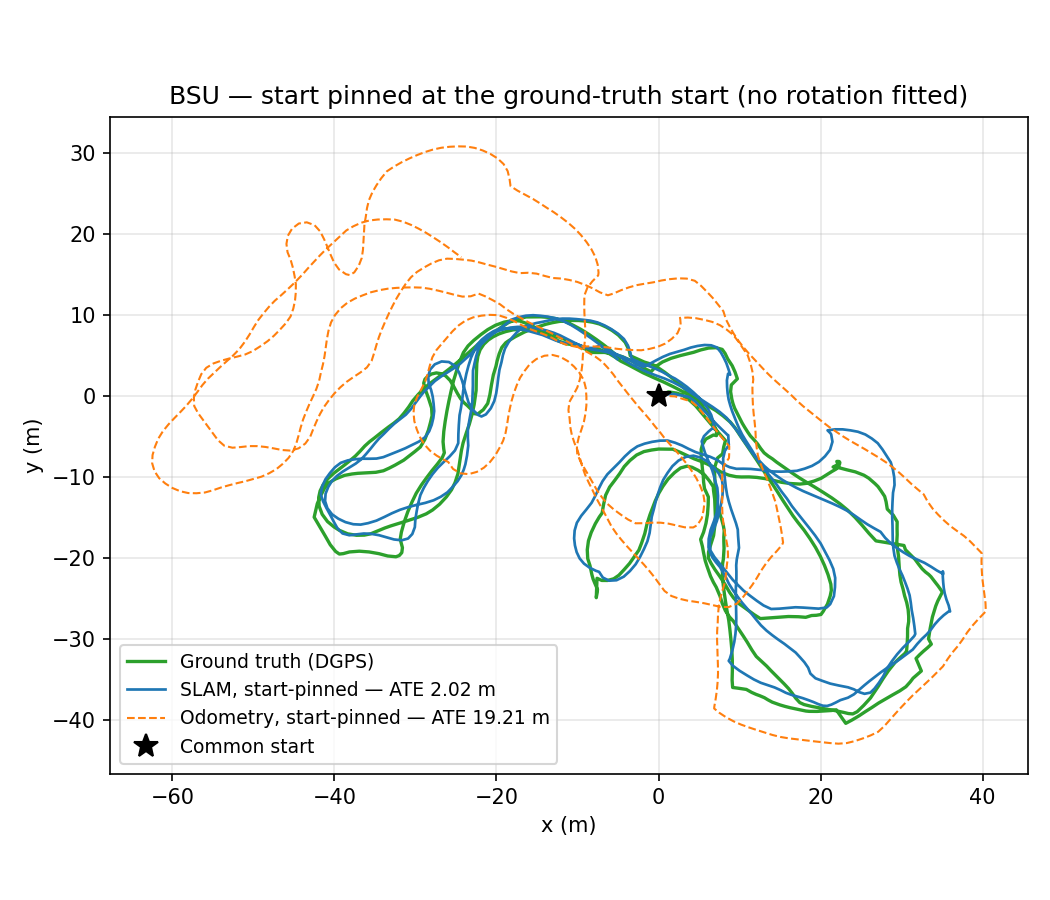
\includegraphics[width=0.72\textwidth]{Image/BSU_traj_origine.png}
\caption{Chapter 2 (run 3, final configuration) — trajectories pinned at the common
start: ground truth, SLAM, pure odometry.}
\label{fig:bsu-traj}
\end{figure}

\begin{figure}[H]
\centering
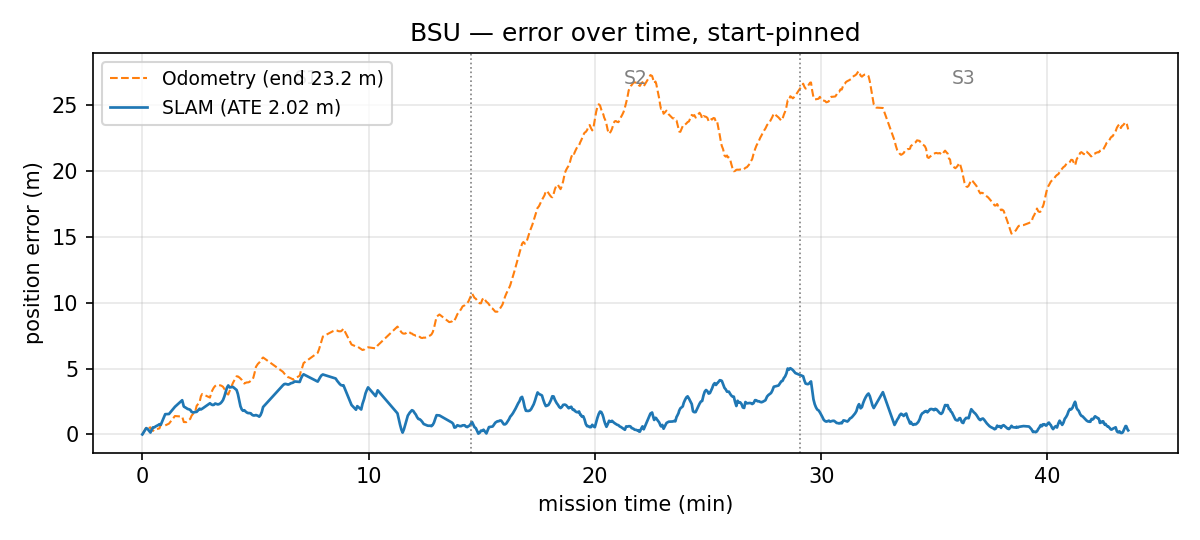
\includegraphics[width=0.9\textwidth]{Image/BSU_err_time_origine.png}
\caption{Chapter 2 — position error over the mission (start-pinned convention).
The Sonar Context loop closures keep the error bounded (ATE 2.02 m over 44 min),
against 19.2 m of accumulated odometry.}
\label{fig:bsu-err}
\end{figure}

\begin{figure}[H]
\centering
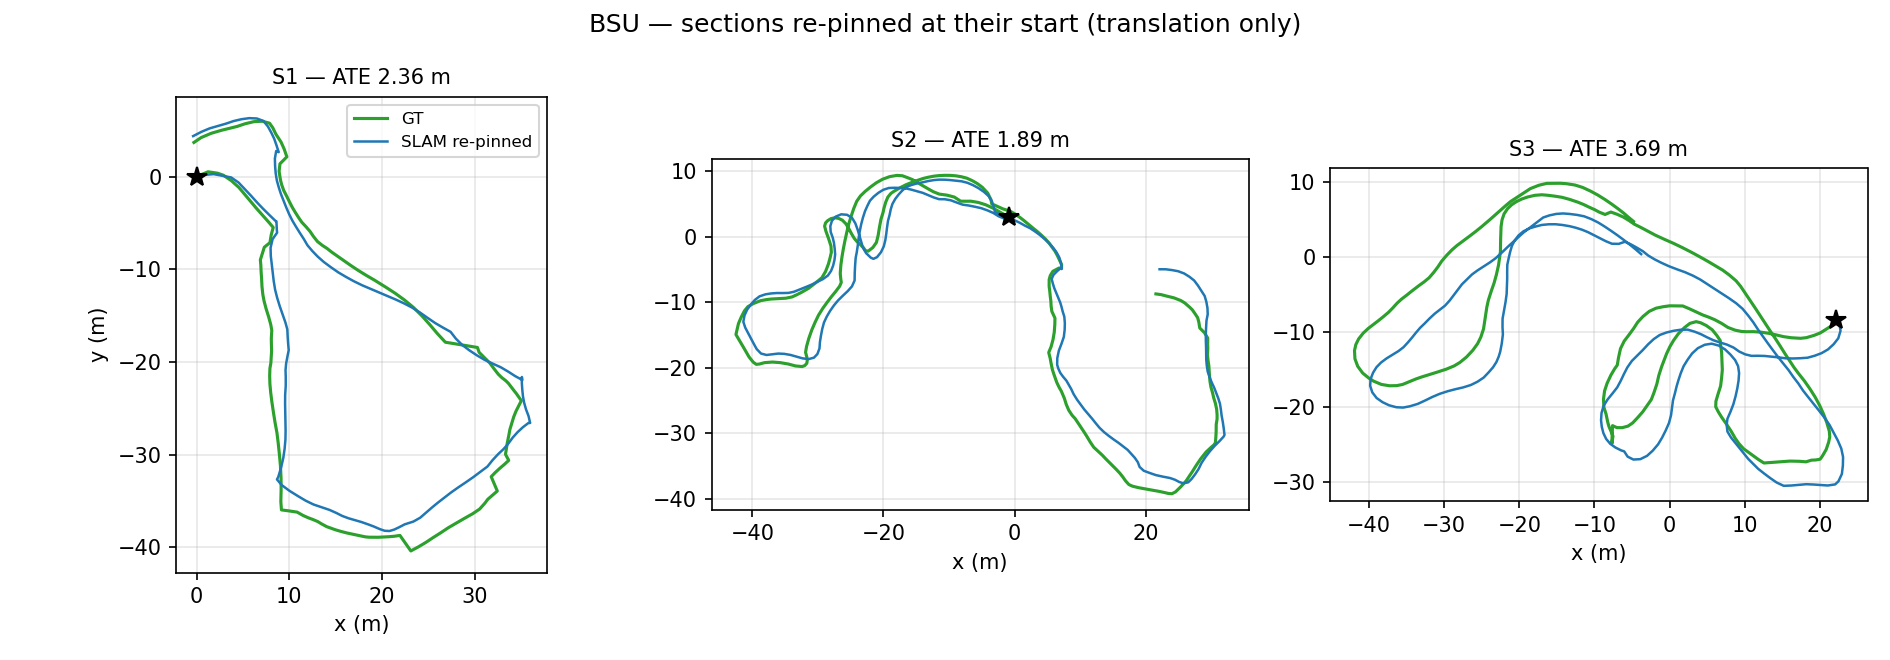
\includegraphics[width=\textwidth]{Image/BSU_sections_origine.png}
\caption{Chapter 2 — sections re-pinned at their start: 1.9--3.7 m,
without any orientation re-fit (§~\ref{sec:protocole}b).}
\label{fig:bsu-sections}
\end{figure}

\begin{figure}[H]
\centering
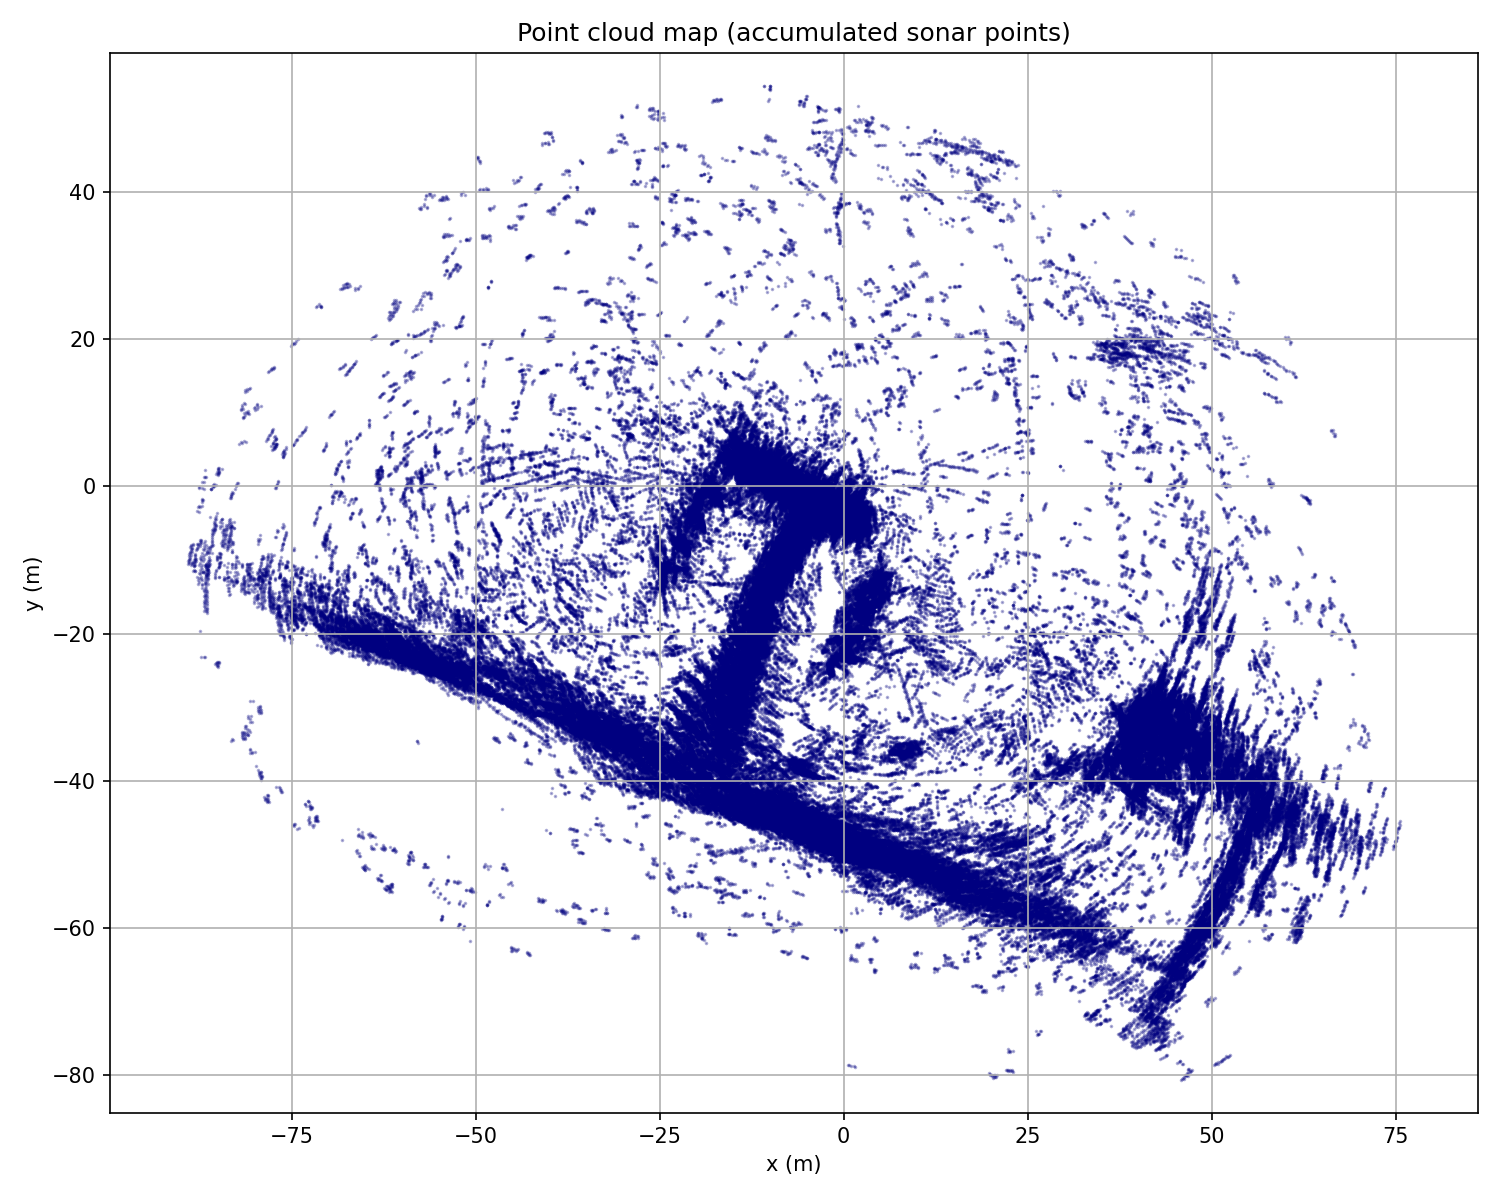
\includegraphics[width=0.8\textwidth]{Image/BSU_pointcloud_map.png}
\caption{Chapter 2 — raw map (full point cloud, no filtering).}
\label{fig:bsu-map}
\end{figure}

\begin{figure}[H]
\centering
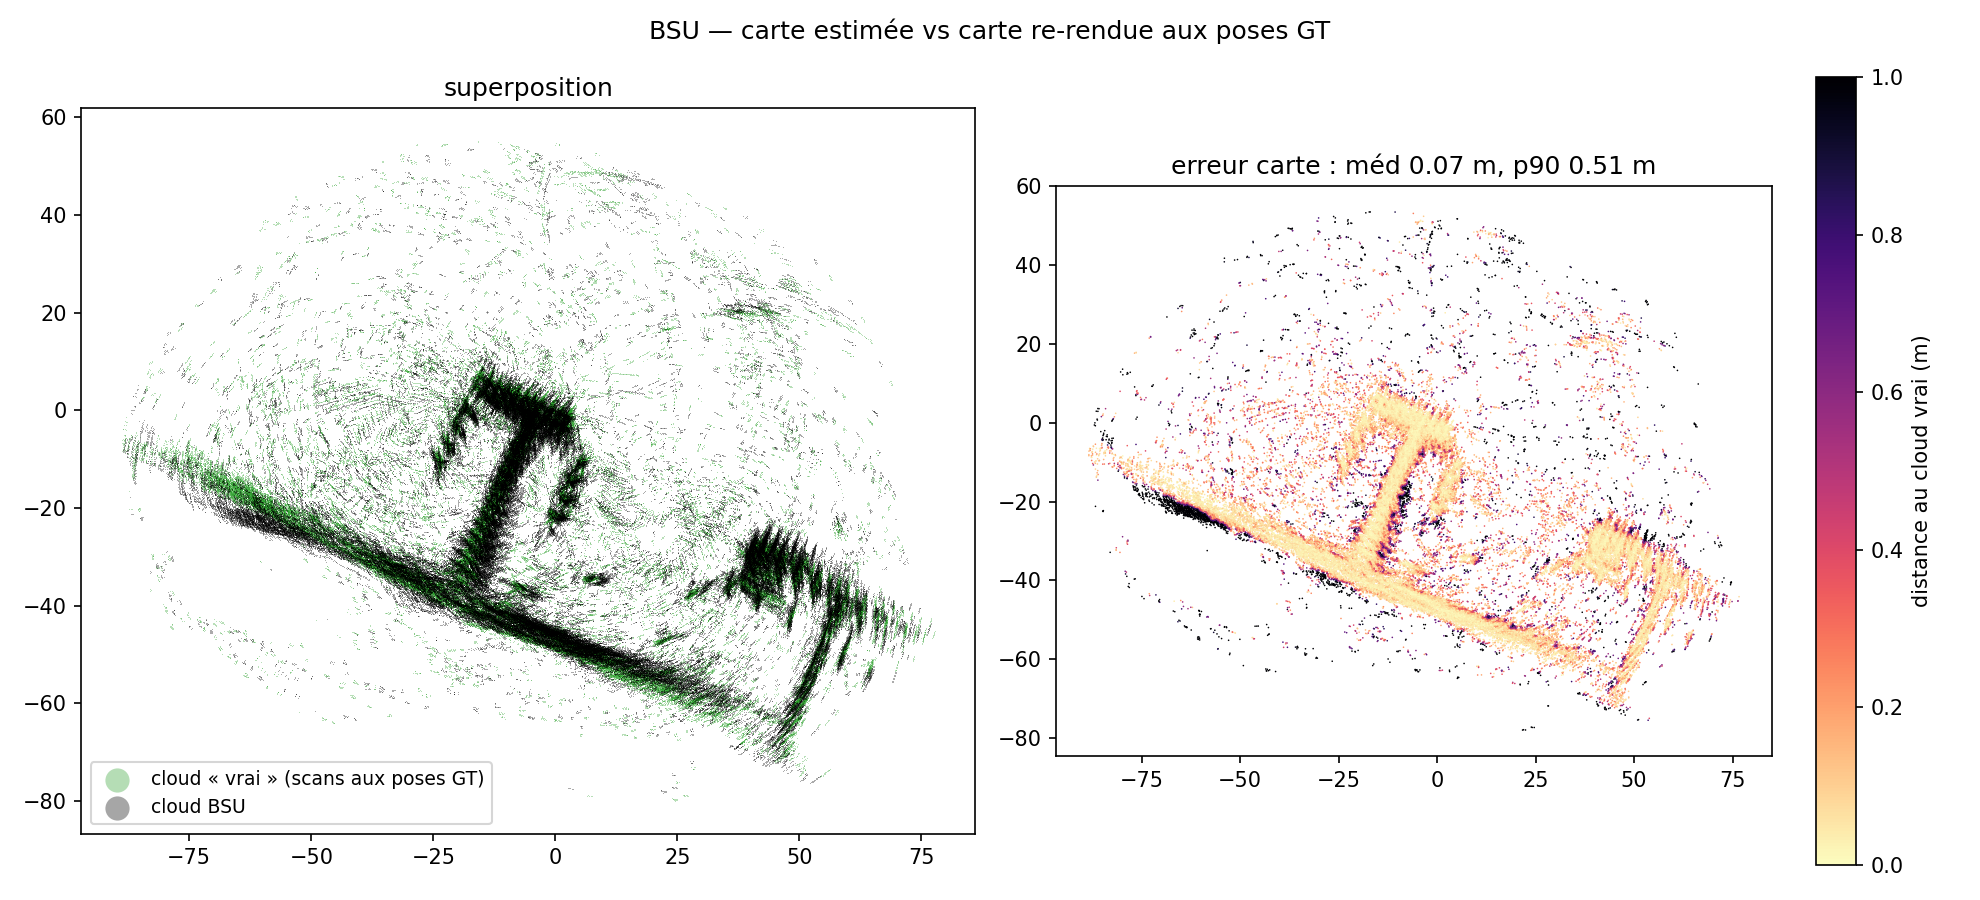
\includegraphics[width=\textwidth]{Image/BSU_cloud_vs_gt.png}
\caption{Chapter 2 — estimated map against the ``true'' map
(§~\ref{sec:protocole}e): median 0.07 m, p90 0.51 m.}
\label{fig:bsu-cloudgt}
\end{figure}

\subsection{Ablation: Sonar Context without the anchor}
\label{sec:sc-noanchor}

We also ran the same pipeline with the USBL factors disabled, everything else
unchanged. The detector itself works: 154 candidates pass the appearance threshold
and the geometric gate, with the same score distribution as in the anchored runs
(median cosine distance 0.60). None of them reaches the graph. The reason is
measured on the retained pairs:
\begin{itemize}
\item without an absolute anchor, the drift accumulated between a place and its
  revisit reaches 9.5 m (median) — 69~\% of the candidates need a correction larger
  than the 8 m guard applied after ICP, and the survivors are too sparse for the
  PCM consistency check;
\item with the USBL factors on, the same detector sees corrections of 1.2 m
  (median, none above the guard) and 65 loops enter the graph.
\end{itemize}
The run without anchor therefore stays at the odometry level (start-pinned ATE
19.24 m against 19.24 m for its odometry). We keep this as a result: appearance
finds the revisits, the anchor keeps the drift inside the domain that the geometric
verification accepts — the two aids are complementary, and neither replaces the
other.

\subsection{Comparison with published methods}
\label{sec:compare}

Same dataset — published rows: Table~I of ISOPoT~[4] (their evaluation toolbox,
sections restarted with the magnetometer heading). Our rows: start-pinned protocol
of §~\ref{sec:protocole}a, \emph{stricter} (no orientation re-fit anywhere).
``Aux'' = auxiliary sensors on top of the sonar.

\begin{table}[H]
\centering
\caption{Comparison on Aracati2017 — section-wise ATE (m) and relative errors.
Best value of each column in bold. Our numbers: chapter-1 champion run and
chapter-2 final run, start-pinned (no orientation re-fit; the published rows
restart each section with the magnetometer heading).}
\label{tab:compare}
\begin{tabular}{llccccc}
\hline
Aux & Method & S1 & S2 & S3 & Trans. (\%) & Rot. (°/m) \\
\hline
None & SONIC~[10] & 36.6 & 113.3 & 69.8 & 137.65 & 2.45 \\
None & ISOPoT~[4] & 8.8 & 12.7 & 16.7 & 22.76 & 0.99 \\
Odom+Mag & Odometry alone (reset/section) & 5.8 & 12.5 & 6.5 & 19.07 & \textbf{0.0} \\
Odom+Mag & DISO~[3] & 5.3 & 6.1 & 10.9 & 13.90 & 0.44 \\
Odom+Mag & SONIC~[10] & 7.0 & 11.2 & 13.7 & 22.83 & \textbf{0.0} \\
Odom+Mag & ISOPoT~[4] & \textbf{3.2} & 3.5 & 4.6 & 9.69 & \textbf{0.0} \\
\hline
Odom+Mag & Our odometry (fixed-heading frame, check) & 6.00 & 12.62 & 8.44 & — & — \\
Odom+USBL & \textbf{Adapted Bruce-SLAM (chap.~1, no USBL)} & 2.57 & 5.61 & \textbf{2.80} & 4.83 & 0.069 \\
Odom+USBL & \textbf{+ Sonar Context (chap.~2)} & \textbf{2.36} & \textbf{1.89} & 3.69 & \textbf{4.73} & 0.096 \\
\hline
\end{tabular}
\end{table}

\noindent Reading, with the precautions of §~\ref{sec:protocole}:

\begin{itemize}
\item \textbf{On the most robust metric (Trans.~\%), we are ahead}: 4.73--4.83~\%
  against 9.69~\% for the best published assisted method (ISOPoT), 13.90~\% for
  DISO.
\item \textbf{Sonar Context is below every published method on all three
  sections} (2.36 / 1.89 / 3.69 m against 3.2 / 3.5 / 4.6 m for the best assisted
  one) — with a stricter protocol on our side (their sections restart with a fresh
  magnetometer heading, ours never re-fit any orientation). Over the \emph{full
  44 min mission}, the start-pinned ATE is \textbf{1.94--2.02 m across three runs}
  — the published odometries have no global figure, since their sections restart
  from zero.
\item \textbf{The raw frame is part of the result}: the chapter~1 USBL variant
  reads 8--11 m in this convention because its noisy heading seed is never
  corrected (§~\ref{sec:chap1-usbl}); with Sonar Context the same convention reads
  1.94--2.02 m, whether the loops straighten a noisy USBL seed (runs 1--2) or the
  frame starts on the measured zero-heading rule (run 3). The ``Odom+Mag'' methods
  start from a magnetometer heading that never drifts.
\item \textbf{The ``Rot. 0.0'' of the Odom+Mag rows is by construction}: their
  heading \emph{is} the magnetometer, which an odometry never modifies; and the
  ``ground-truth'' heading of this dataset derives from the same compass (verified in
  the bag: $\int\omega_z$ and $\Delta$yaw of the ground truth identical to 0.01° over
  120 s). Our 0.057--0.090 °/m are not ``worse'': SLAM adjusts the heading through
  the loops, for global consistency.
\item \textbf{Protocol check}: our odometry evaluated in a fixed-heading frame
  (6.00 / 12.62 / 8.44 m) lands close to their published ``odometry alone'' row
  (5.8 / 12.5 / 6.5 m) on the same data — the two evaluations are consistent.
  Remaining difference: their odometry restarts from zero at each section, ours
  runs for 44 min straight and closes loops across sections. Finally, none of the
  published methods delivers a map — we deliver trajectory \emph{and} map (0.07 m
  median, figure~\ref{fig:bsu-cloudgt}).
\item \textbf{Nature of the methods}: ISOPoT relies on pre-trained networks (TAPNext
  point tracking, ResNet50 descriptors) with GPU inference; our two methods are
  100~\% geometric (CFAR, ICP, factor graph), with no learning, CPU-executable —
  embeddable.
\end{itemize}
